\documentclass[11pt,a4paper]{article}
\usepackage[top=3cm, bottom=2cm, left=2cm, right=2cm]{geometry}
\usepackage[utf8]{inputenc}
\usepackage{amsmath, amsfonts, amssymb}
\usepackage{siunitx}
\usepackage[brazil]{babel}
\usepackage{graphicx}
\usepackage[margin=10pt,font={small, it},labelfont=bf, textfont=it]{caption}
\usepackage[dvipsnames, svgnames]{xcolor}
\DeclareCaptionFont{MediumOrchid}{\color[svgnames]{MediumOrchid}}
\usepackage[pdftex]{hyperref}
\usepackage{natbib}
\bibliographystyle{plainnat}
\bibpunct{[}{]}{,}{s}{}{}
\usepackage{color}
\usepackage{footnote}
\usepackage{setspace}
\usepackage{booktabs}
\usepackage{multirow}
\usepackage{subfigure}
\usepackage{fancyhdr}
\usepackage{leading}
\usepackage{indentfirst}
\usepackage{wrapfig}
\usepackage{mdframed}
\usepackage{etoolbox}
\usepackage[version=4]{mhchem}
\usepackage{enumitem}
\usepackage{caption}
\usepackage{titlesec}
\usepackage{tcolorbox}
\usepackage{tikz}
\usepackage{LobsterTwo}
\usepackage[T1]{fontenc}
\usepackage{fontspec}
\usepackage{txfonts}
\AtBeginEnvironment{equation}{\fontsize{13}{16}\selectfont}


\titleformat{\section}{\LobsterTwo\LARGE\color{CarnationPink}}{\thesection.}{1em}{}
\titleformat{\subsection}{\LobsterTwo\LARGE\color{CarnationPink}}{\thesubsection}{1em}{}


\DeclareCaptionLabelFormat{figuras}{\textcolor{DarkTurquoise}{Figura \arabic{figure}}}
\captionsetup[figure]{labelformat=figuras}

\makeatletter
\renewcommand\tagform@[1]{\maketag@@@{\color{CarnationPink}(#1)}}
\makeatother

\renewcommand{\theequation}{Eq. \arabic{equation}}
\renewcommand{\thefigure}{Fig. \arabic{figure}}
\renewcommand{\thesection}{\textcolor{CarnationPink}{\arabic{section}}}

\setlist[itemize]{label=\textcolor{CarnationPink}{$\mathbf{\square}$}}

\setlist[enumerate]{label=\textcolor{CarnationPink}{\arabic*.}, align=left}


\newcounter{exemplo}

\NewDocumentEnvironment{exemplo}{ O{} }{%
\allowbreak
\setlength{\parindent}{0pt}
  \begin{mdframed}[
  leftline=true,
  topline=false,
  rightline=false,
  bottomline=false,
  linewidth=2pt,
  linecolor=CarnationPink,
  frametitlerule=false,
  frametitlefont=\LobsterTwo\large\color{CarnationPink},
  frametitle={\color{CarnationPink}\LobsterTwo\large #1},
  ]
}{%
  \end{mdframed}
}

\setlength{\fboxsep}{5pt}
\setlength{\fboxrule}{1.5pt}
\usepackage{float}
\renewcommand{\thefootnote}{\alph{footnote}}
\usepackage{url}
\hypersetup{
	colorlinks=true,
	linkcolor=DarkTurquoise,
	filecolor=DarkTurquoise,      
	urlcolor=DarkTurquoise,
	citecolor=DarkTurquoise,
	pdftitle={Especialista em Física da Radioterapia}
}
\pagestyle{fancy}
\fancyhf{}
\renewcommand{\headrulewidth}{0pt}
\rfoot{Página \thepage}

\title{\LobsterTwo\Huge{Braquiterapia}}
\author{\LobsterTwo\Large{Braquiterapia Oftalmológica}}
\date{\LobsterTwo\textit{Dalila Mendonça}}
\begin{document}
	\maketitle

    \section{Braquiterapia Oftalmológica}


    A braquiterapia oftamológica é utilizada para o tratamento de Melanomas Oculares ou melanomas coroidais e em retinoblastomas (mais comum em pacientes neonatais e bebês). Os possíveis tratamentos para melanomas oculares são a enucleação (retirada do olho) ou a braquiterapia com placas oftamológicas. 
    
    Os primeiros tratamentos de braquiterapia oftalmológica eram realizados com Cobalto-60 e subsequentemente foram testadas outras fontes como o Irídio-192, Rutênio-106, Iodo-125  Paládio-103, Estrôncio-90 e Césio-131. Antes de 2002 os guidelines eram focados no Iodo-125 mas conforme outras fontes foram sendo utilizadas, novos protocolos foram estabelecidos pela American Brachyterapy Society. Collaborative Ocular Melanoma Study (COMS) é um ensaio clínico multi disciplinar que desenvolveu estudos randomizados e padronizou as placas de braquiterapia para o tratamento de melanomas coroidais.


    \subsection{Critério de Exclusão}

    Tumores com extensão extraoculares grosseiras (T4e ou maior de 5cm), diâmetros basais que excedem os limites de braquiterapia estabelecidos pelo tamanho das placas oftalmológicas e olho doloroso cego e sem percepção de luz.

\subsection{Possíveis reações}


    \begin{itemize}
        \item Efeitos tardios - predominantes: Retinopatia radio-induzida, catarata, necrose escleral, Vazamento vascular periférico da retina com exsudação e hemorragia.
        \item Tumores próximos a fóvea ocular e ao nervo ótico podem causar morbidades como a cegueira. Quanto maior a distância entre a placa e a mácula ou o nervo ótico melhor o resultado visual.
        \item É possível evitar a incidência de retinopatia por radiação e neuropatia ótica aplicando injeções intravítreas de triancinolona e agentes anti-fator de crescimento endotelial vascular
    \end{itemize}


\subsection{Planejamento de Tratamento} 


    \begin{itemize}
        \item É necessário informações do oftalmologista quanto à lateralidade, estágio, tamanho do tumor (diâmetro e altura) que devem ser confirmados através de uma ultrassom e um diagrama de fundo detalhado contendo a localização do tumor, medidas tumorais assim como a distância do tumor até a fóvea, nervo ótico, glândula lacrimal,  cristalino e o olho oposto.
        \item os dados do diagrama de fundo são transferidos para o TPS e é inserido os dados dosimétricos da fonte de radiação escolhida para o procedimento e então a dose no tumor e a dose nos OAR são calculadas com base na COMS e no TG-129.
        \item Os diâmetros do tumor devem ser menores que o PTV ou o diâmetro da placa para evitar perca geográfica.
        \item O ponto de prescrição deve ser no ápice do tumor, que é o ponto de espessura máxima.
        \item A isodose de prescrição deve cobrir todo o tumor para maximizar o controle local.
        \item A prescrição de dose para o Retinoblastoma é de 40Gy a 45Gy entre 1 - 5 dias.
        \item A dose total no ápice tumoral pode variar, dependendo do radionuclídio escolhido, entre 70 Gy a 100 Gy nos casos de melanoma.
        \item A prescrição de Dose comum para o Melanoma Coróide é de 85 Gy em um mínimo de 5 mm de profundidade utilizando uma placa oftalmológica com 0.2 cm de margem em torno do diâmetro basal do tumor, que deve ser entregue entre 3 a 7 dias consecutivos.
        \item Existe um gradiente de dose e portanto a dose máxima pode variar com a profundidade de tratamento e dependendo do Radionuclídio utilizado.
        \item Esta prescrição em um meio homogênio entrega 75Gy a 5mm de profundidade para o \ce{^{125}I} e 69 Gy a 5 mm de profundidade para o \ce{^{103}Pd}.
        \item Para o I-125: A prescrição de 85Gy a  10 mm terá Dmax (inner-scleral) de 644 Gy, a 3 mm Dmax = 166 Gy e a  5mm Dmax  é 260 Gy.
        \item Emissores Beta (Ru-106 e Rh 106): 5mm dmax = 800 Gy, são indicados para tratar lesões com espessura do ápice menor que 5 - 6 mm
        \item As placas de 106-Ru são finas, em torno de 1 mm
        \item \ce{^{103}Pd} com energia de 21 Kev, \ce{^{125}I} com energia de 28Kev e \ce{^{131}Cs} com energia de 30 Kev: aumenta progressivamente o gradiente de dose do menor para o maior; Aumenta a dose na esclera e diminui nas estruturas oculares normais.
        \item Métodos de cálculos heterogêneos acarretam em uma diferença de dose superior a 10\% comparado aos cálculos em meios homogêneos;
        \item A taxa de dose não deve ser menor que o padrão COMS equivalente de 0.60Gy/h para o \ce{^{125}I}.
        \item A atividade típica de \ce{^{125}I} utilizada por semente varia entre 0.5 - 5 mCi para alcançar taxas de dose ente 0.5 - 1.25Gy/h
        \item A localização do tumor pode ser feita utilizando fundoscopia, fotografia  de fundo e ultrassom. CT e RM podem ser utilizadas para a localização da lesão. Pós implante, a verificação da posição das placas é feita com ultrassom.
        \item Além das fontes já citadas, podem ser utilizadas \ce{^{90}Sr} e \ce{^{90}Y} (emissores beta) e o \ce{^{60}Co}.
    \end{itemize}


    \subsection{Cirurgia}

        Recomenda-se uma equipe multidisciplinar de oncologista oftalmológico, radio-oncologista e físico médico. O tumor é localizado pelo cirurgião e é medido para identificar qual diâmetro de placa será utilizado, que deve considerar o diâmetro do tumor e a margem de planejamento. Na sequência a placa ocular é afixada na ésclera ( tecido fibroso que reveste o olho) através de suturas e caso algum músculo ocular esteja impedindo a inserção da placa ele é realocado. O tempo de inserção é registrado no report e um tapa olho de chumbo é colocado sobre o olho afetado. Em seguida a placa permanece no local durante todo o tempo pré-planejado para fornecer a dose apropriada na profundidade e em seguida a placa é removida sob anestesia local e qualquer músculo ocular que tenha sido realocado para conseguir inserir a placa é colocado em seu lugar novamente.


    \begin{figure}[h]
        \centering
        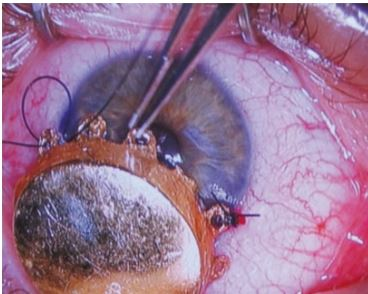
\includegraphics[width=0.5\textwidth]{Imagens/placaComsOuroMC.JPG}
        \caption{Fotografia externa da placa COMS feita de uma liga de ouro, costurada na esclera após a localização.}
    \end{figure}
 


    \begin{figure}[h]
        \centering
        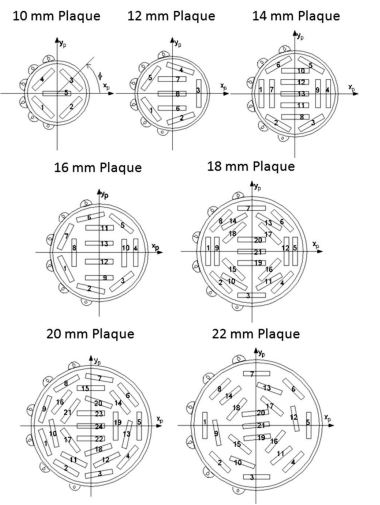
\includegraphics[width=0.4\textwidth]{Imagens/placasComs.JPG}
        \caption{Diagrama das sementes distribuídas em placas COMS. Consistem em um suporte feito de uma liga de ouro com um portador de sementes feitos de Silastic(borracha de silicone) acoplados no suporte.}
    \end{figure}


    \begin{figure}[h]
        \centering
        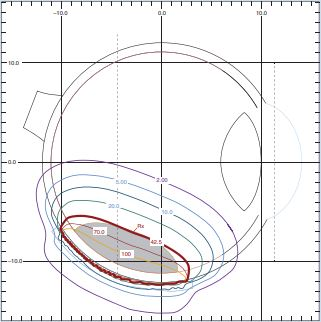
\includegraphics[width=0.45\textwidth]{Imagens/distribDosePlacaOftamRutenio.JPG}
        \caption{Distribuição de Isodose para uma Placa de Rutênio de 15.3mm modelo CCA, onde o alvo é a sombra cinza. Devido ao acentuado falloff de dose a profundidade de tratamento dessas placas são limitadas entre 5-6 mm a partir da superfície da placa.}
    \end{figure}
 


    \begin{figure}[h]
        \centering
        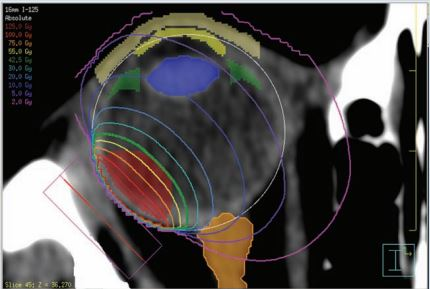
\includegraphics[width=0.5\textwidth]{Imagens/distribDosePlacaComsI125.JPG}
        \caption{Corte axial de TC mostrando a distribuição de isodose para uma placa de Iodo-125 COMS de 16 mm para entregar 42.5Gy no alvo (em vermelho). O perfil de dose baseado em Monte-Carlo, que considera os efeitos da capa de ouro e a atenuação nos portadores de silicone, foi atribuído à fonte, representada pelo retângulo.}
    \end{figure}
 

% TODO: pegar dados no TG 129 e no guideline da ABS



\end{document}
